% Chapter 11 -- translated by Claude (2026), continuing the voice and
% register of the Burkett-Hutcheson chapters.

\chapter{Simulation in the time domain}

\section{Relation between FD and TR}

In this chapter, we will see the simulation techniques for analysis
in the time domain, that is, transient analysis, in Symbulator.
There is an intimate relation between analysis in the frequency
domain (FD) and analysis in the time domain (TR). In TR, Symbulator
uses the techniques of the Laplace transform to obtain the complete
answers in the time domain, from the frequency-domain answers
obtained with FD. The complete answer includes the forced response
and the transient response. As we have learned in the classroom, the
Laplace transform can take an answer from the frequency domain to
the time domain.

\subsection{DiffEq}

Symbulator uses the powerful program DiffEq, written by Lars
Frederiksen, who is the best calculator programmer I have known, and
my personal friend. DiffEq is a group of programs made to solve
differential equations. The most advanced Laplace transform tool for
TI calculators is called Advanced Laplace, also made by Lars
Frederiksen. Although less powerful, the Laplace transform of DiffEq
is faster than that of Advanced Laplace. That is why Symbulator
prefers DiffEq.

Symbulator uses the \code{laplace} function of DiffEq at the start
of any FD or TR simulation, and the \code{ilaplace} function of the
same at the end of any TR simulation. That is why it is necessary to
have this program installed when Symbulator is used to perform these
two types of analysis.

\section{Two ways to obtain answers in the time domain}

There are two ways for the Symbulator user to obtain answers in the
time domain:

The first alternative (see section 11.3) is to run an analysis in
the frequency domain, and then convert the answers that interest us
to the time domain. This analysis is done using the
\code{sq\char`\\fd} door. This analysis solves the circuit in the
frequency domain, converting all the values of sources that are in
the time domain to their equivalents in the frequency domain, but it
does not convert the answers to the time domain. It will give us all
the answers in the frequency domain. Since no automatic conversion
of all the answers to the time domain is done, all the time these
conversions would have consumed is saved. So, the simulation will
take the minimum possible. After the analysis, you can take to the
time domain those answers that interest you. This alternative should
be used in two cases: a) when we want answers both in the time
domain and in the frequency domain, and b) when we want the fastest
possible simulation, and we want only some answers in the time
domain, not the whole set.

The second alternative (from section 11.5 onward) is to run a
transient analysis. This analysis is done using the
\code{sq\char`\\tr} door, whose use we will explain later. This
analysis solves the circuit in the frequency domain, converting all
the values of sources that are in the time domain to their
equivalents in the frequency domain, and finally converts all the
answers back to the time domain. This analysis will give us all the
answers in the time domain. The user never sees the answers in the
frequency domain. The conversion of all the answers to the time
domain can consume several minutes, the more the larger the circuit.
Therefore, this alternative should be used only in three cases: a)
when the circuit is small, b) when the user is interested in all the
answers in the time domain and not only in some answers, and c) when
the user does not mind the simulation taking a few minutes.

\section{Two ways to convert answers to the time domain}

When we use the first alternative, we will have to convert the
answers that interest us to the time domain ourselves. We can do it
in two ways.

\subsection{The ilaplace function of DiffEq}

DiffEq converts a function from the frequency domain to the time
domain, using the \code{ilaplace} function, like this:

\begin{entry}
dif\ilaplace(function of the frequency,s)
\end{entry}

It is worth pointing out that DiffEq also does the inverse
operation, that is, converting a function from the time domain to
the frequency domain, using the \code{laplace} function, like this:

\begin{entry}
dif\laplace(function of time,t)
\end{entry}

\subsection{The fd\_to\_tr tool of Symbulator}

The \code{fd\_to\_tr} tool of Symbulator is really a kind of
shortcut for the use of the \code{ilaplace} function of DiffEq. The
only purpose of this tool is to save the user from placing the
\code{,s)} at the end of the command line. It is the \code{ilaplace}
function that does all the work. This tool is used like this:

\begin{entry}
sq\fd_to_tr(answer in the frequency domain)
\end{entry}

It gives us the answer in the time domain.

\section{The Symbulator menu}

Symbulator includes a program to create a personalized menu, called
in English a Custom Menu. The program is executed like this:

\begin{entry}
sq\makemenu()
\end{entry}

When executed, this program will create a personalized menu, in
which all the doors, tools and elements of Symbulator can be found.
This way, you will avoid having to type the names of the tools and
doors, since you can select them using the cursor keys.

For information on how to restore the original menu of the
calculator, read the User's Manual.

\section{Door for the time domain: tr}

If we choose the second alternative, that is, to run a simulation in
the time domain $t$, we will use the door called
\code{sq\char`\\tr}.

\section{Input data}

The only input data that must be given to this door is the circuit
description, using the same notation used for a simulation in the
frequency domain. The time domain simulation is ordered like this:
\code{sq\char`\\tr(circuit)}.

\section{Initial conditions}

Just as in the frequency domain simulation, the fifth term in the
description of an inductor or a capacitor is its initial condition.

\section{Answers}

In the case of the time domain simulation, the answers are: the node
voltages, the voltage drops in the elements and the currents in the
elements. The powers consumed by the elements are not given. As we
already explained in section 11.2, all these answers will be
delivered in the time domain. Therefore, they will be symbolic
expressions as functions of time $t$.

Let us now see several problems that illustrate how transient
analysis problems are solved in Symbulator.

\problem{075}

\emph{Problem: a) According to the figure, find the ratio
$I_L(s)/V_s(s)$. b) Make $v_s(t) = 100u(t)$~V and find $i_L(t)$.}


% figures added 10 Sep 2026
\begin{figure}[!ht]
\centering
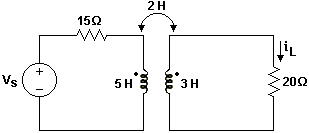
\includegraphics[width=105mm]{book_figures/p075_0.png}
\caption*{Circuit for Problem 075}
\end{figure}

Solution: Since the problem does not specify initial conditions, nor
gives us the way to calculate them, we assume they are null. This
problem has two parts. The first asks us for an answer in the
frequency domain, while the second asks us for an answer in the time
domain. There are two good reasons to solve this problem using the
first alternative. (As we explained in section 11.2, the first
alternative consists of simulating with \code{sq\char`\\fd} and then
transforming with \code{sq\char`\\fd\_to\_tr}.) The first reason is
that we are interested in only one answer in the time domain. The
second reason is that we are also interested in an answer in the
frequency domain. As we explained in section 11.2, both reasons are
sufficient cause to use the first alternative instead of the second.
Below, the procedure to solve this problem.

For the purposes of answering the first question, it does not matter
what value we assign to the voltage source. We could define its
value as \code{vs}, or as \code{100u(t)}, and the answer would be
the same. This is because the answer is a ratio, and the source will
influence both the numerator and the denominator, canceling its
effect. Now, if at the beginning we use a value like \code{vs}, when
we go to answer the second question, we will have to simulate again
using the new value of \code{100u(t)}. However, if at the beginning
we use the value of \code{100u(t)}, this single simulation will
serve us to answer both questions. So, we take advantage of the fact
that the first question allows it, and use the value of the source
as \code{100u(t)}. It is necessary to say that the \code{ilaplace}
function of the DiffEq program understands what $u(t)$ and
$\delta(t)$ mean. In fact, this function assumes that any numerical
value entered is multiplied by $u(t)$. Therefore, it is not
necessary to enter the value \code{100u(t)}, because for
\code{ilaplace}, saying 100 and saying $100u(t)$ is the same. Below,
the description:

\begin{entry}
sq\fd("e1,1,0,100,0;r1,1,2,15,0;r2,3,0,20,0;l1,2,0,5,0;
      l2,3,0,3,0;m1,l1,l2,2,0")
\end{entry}

With \key{ENTER}, the simulation executes. To answer the first
question, we request the ratio \code{ir2/v1} and obtain
\code{2*s/(11*s\^{}2+145*s+300)}. To answer the second question, we
use \code{sq\char`\\fd\_to\_tr(ir2)} and obtain:

\begin{entry}
40*√313*e^((5*√313/22-145/22)*t)/313
   -40*√313*e^((-5*√313/22-145/22)*t)/313
\end{entry}

These are the correct answers. Do you wish to see the answers in
approximate form? If we request \code{approx(ans(1))}, we will
obtain \code{2.26*(.0765)\^{}t-2.26*(2.46E-5)\^{}t} (rounding). If
we request \code{expand(ans(1))}, we will obtain
\code{2.26/(e\^{}t)\^{}(2.57)-2.26/(e\^{}t)\^{}(10.6)} (rounding).
Let us learn more about this behavior of approximate answers.

\section{Approximate presentation with exponentials}

When the Exact/Approx mode is in AUTO, the calculator will keep an
expression in the form $e^{nt}$ only if $n$ is an exact number. For
example, if we enter \code{e\^{}(2t/3)} in the entry line, we will
see that in the history area the calculator also presents us
\code{e\^{}(2t/3)}. This is because the number that accompanies $t$,
that is, 2/3, is an exact number.

The disadvantage of this exact way of presenting the answer resides
in the fact that on some occasions, as in the case of the problem we
just solved, the exact expression is so voluminous that its use is
uncomfortable. Furthermore, some textbooks and professors favor
answers in approximate presentation.

If $n$ is an approximate number, the calculator will convert the
expression to a totally approximate value, to the point of
eliminating the exponentials. For example, let us use the expression
in approximate form, either by entering \code{e\^{}(2t/3.)} or
\code{approx(e\^{}(2t/3))} in the entry line (both the point and the
\code{approx} command have the effect of turning the expression
approximate). We will see that in the history area the calculator
now presents us \code{(1.94773404)\^{}t}. This is because the number
that accompanies $t$, that is, 2/3., is an approximate number.

The disadvantage of this totally approximate way of presenting the
answer resides in the fact that the exponentials have been replaced,
diluted in the approximate number of the base. In the years I have
been studying electrical engineering, I have never seen a textbook
or a professor who favors the use of answers in this approximate
presentation without exponentials.

Therefore, it is desirable to obtain a combination of the virtues of
both ways: an approximate expression that is smaller than the exact
one, but that keeps the exponentials in their place. In the
calculator, it is possible to obtain this type of answer, using the
\code{expand} command. This command is used like this:
\code{expand(expression,variable)}, and its result is that the
expression will be shown in an expanded way, with respect to the
variable. In our example, if we enter \code{expand(e\^{}(2t/3.),t)}
or \code{expand(approx(e\^{}(2t/3)),t)} in the entry line, we will
see that in the history area the calculator presents us
\code{(e\^{}t)\^{}.666666667}.

Also in this case, we would prefer a somewhat different
presentation, like the following: $e^{.666666667t}$. Even so, that
presentation is much better than the two previous ones.

If we expand an exponential expression whose number $n$ is negative,
the \code{expand} command will show an interesting behavior. For
example, with \code{expand(e\^{}(-2t/3.),t)} in the entry line, we
will see that in the history area the calculator presents us
\code{1/(e\^{}t)\^{}.666666667}.

Certainly, we would prefer a different presentation, like the
following: $e^{-.666666667t}$. But having the first expression, we
can obtain the second easily.

\problem{076}

\emph{Problem: a) For the circuit shown in the figure, find
$H(s) = v_{C2}/v_S$. b) Let $v_{C1}(0^{+}) = 0$ and
$v_{C2}(0^{+}) = 0$. Find $v_{C2}(t)$ if $v_S(t) = u(t)$.}


% figures added 10 Sep 2026
\begin{figure}[!ht]
\centering
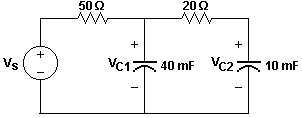
\includegraphics[width=103mm]{book_figures/p076_0.png}
\caption*{Circuit for Problem 076}
\end{figure}

Solution: The problem clearly specifies that the initial conditions
are null. Since this problem is identical to the previous one, we
save ourselves the explanations, which would be redundant. We will
only say that, for DiffEq, and therefore for Symbulator, $u(t)$ is
the same as 1:

\begin{entry}
sq\fd("es,1,0,1,0;r1,1,2,50,0;r2,2,3,20,0;cc1,2,0,.04,0;
      cc2,3,0,.01,0")
\end{entry}

With \key{ENTER}, the simulation executes. To answer the first
question, we request the ratio \code{v3/v1} and obtain
\code{2.5/(s\^{}2+6.75*s+2.5)}. To answer the second question, we
use \code{expand(sq\char`\\fd\_to\_tr(v3),t)} and obtain
\code{-1.066/(e\^{}t)\^{}(.393)+.0659/(e\^{}t)\^{}(6.36)+1.}
(rounding).

Instead of having used
\code{expand(sq\char`\\fd\_to\_tr(v3),t)}, we could have used first
\code{sq\char`\\fd\_to\_tr(v3)} and then \code{expand(ans(1),t)},
and the result would be the same.

\section{Intervals and simulations}

In Symbulator, each interval of time requires one simulation. To
simulate the behavior of a circuit that has a switch, which switches
at a given time, say $t = 0$, we must do two simulations: one for
$t < 0$ and another for $t > 0$.

The same principle governs the function $u(t)$. Mathematically,
$n \cdot u(t)$ indicates that for times $< t$ the function is worth
0, and for times $> t$ the function is worth $n$. In the same way,
mathematically, $n \cdot u(-t)$ indicates that for times $< t$ the
function is worth $n$, and for times $> t$ the function is worth 0.
For the purposes of the simulation, the $u(t)$ does not have that
meaning. We must perform one simulation for each interval of time.

Let us see several examples.

\problem{077}

\emph{Problem: After remaining closed for a long time, the switch in
the circuit of the figure opens at $t = 0$. a) Find $i_L(t)$ for
$t > 0$. b) Evaluate $i_L(10~\mathrm{ms})$. c) Find $t_1$ if
$i_L(t_1) = 0.5\,i_L(0)$.}


% figures added 10 Sep 2026
\begin{figure}[!ht]
\centering
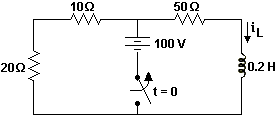
\includegraphics[width=95mm]{book_figures/p077_0.png}
\caption*{Circuit for Problem 077}
\end{figure}

Solution: The problem tells us that there is a switch that switches
at $t = 0$. We must first run a simulation, in direct current, for
$t < 0$, which will allow us to find the initial condition of the
inductor. Then we will run a second simulation, in the frequency
domain, for $t > 0$, to answer the questions. The procedure is the
following:

\begin{entry}
sq\dc("r1,1,0,20;r2,2,1,10;r3,2,3,50;l1,3,0,.2;e1,2,0,100"):il1
\end{entry}

We request the direct current simulation, and immediately after ask
for the current in the inductor. With \key{ENTER}, the simulation
executes. We obtain 2 as the current in the inductor. This will be
its initial condition for the simulation of the next interval:

\begin{entry}
sq\fd("r1,1,0,20,0;r2,2,1,10,0;r3,2,3,50,0;l1,3,0,.2,2"):
sq\fd_to_tr(il1)
\end{entry}

We request the simulation in the frequency domain, and immediately
after ask for the current in the inductor, in the time domain. With
\key{ENTER}, the simulation executes. We obtain
\code{2*e\^{}(-400*t)} as the expression for the current in the
inductor. This answers question a).

To answer question b), we use \code{ans(1)|t=10E-3} and obtain
.0366 (rounding).

To answer question c), we use \code{solve(ans(2)=.5*2,t)}. Note that
the command means: ``Tell me how much time is worth when the
expression \code{2*e\^{}(-400*t)}, recalled by \code{ans(2)}, equals
0.5 times the initial current, which is 2.'' We obtain
\code{t}~$= .00173$ (rounding).

In summary, this problem did not give us the initial conditions, but
gave us a way to calculate them by means of a direct current
simulation for before the switch switched. This problem required two
simulations, one for each interval of time.

\problem{078}

\emph{Problem: If $i_L(0) = 10$~A in the circuit of the figure, find
$i_L(t)$ for $t > 0$.}


% figures added 10 Sep 2026
\begin{figure}[!ht]
\centering
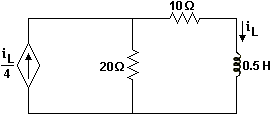
\includegraphics[width=93mm]{book_figures/p078_0.png}
\caption*{Circuit for Problem 078}
\end{figure}

Solution: The problem gives us the initial condition of the
inductor. Therefore, we only need to run one simulation:

\begin{entry}
sq\fd("j1,0,1,il/4,0;r1,1,0,20,0;r2,1,2,10,0;l,2,0,.5,10"):
sq\fd_to_tr(il)
\end{entry}

We request the simulation in the frequency domain, and immediately
after ask for the current in the inductor in the time domain. With
\key{ENTER}, the simulation executes. We obtain
\code{10*e\^{}(-50*t)} as the expression for the current in the
inductor.

This problem gave us the initial conditions. It only required one
simulation.

\problem{079}

\emph{Problem: a) Find $v_C(t)$ for $t > 0$. b) At what time is
$v_C = 0.1\,v_C(0)$?}


% figures added 10 Sep 2026
\begin{figure}[!ht]
\centering
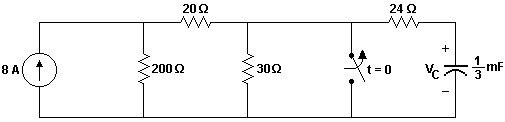
\includegraphics[width=150mm]{book_figures/p079_0.png}
\caption*{Circuit for Problem 079}
\end{figure}

Solution: This problem is similar to Problem 076. We prefer to use
exact values:

\begin{entry}
sq\dc("j1,0,1,8;r1,1,0,200;r2,1,2,20;r3,2,0,30;r4,2,3,24;
      c,3,0,(1/3)/1000"):vc
\end{entry}

We simulate in direct current, and ask for the voltage in the
capacitor. We press \key{ENTER}. We obtain 192 as the voltage in the
capacitor. This will be its initial condition for the simulation of
the next interval. We simulate in the frequency domain, and ask for
the voltage in the capacitor, in the time domain:

\begin{entry}
sq\fd("j1,0,1,8,0;r1,1,0,200,0;r2,1,2,20,0;r3,2,0,30,0;
      r4,2,3,24,0;c,3,0,(1/3)/1000,192;s1,2,0,0,0"):
sq\fd_to_tr(vc)
\end{entry}

Note that to simulate the closed switch, we used a short circuit. We
could have eliminated the part of the circuit that is to the left of
the switch, since it does not interest us. That way we would save
the simulator work. But we will be rigorous, and leave it. We press
\key{ENTER}. We obtain \code{192*e\^{}(-125*t)}. This answers
question a).

To answer question b), we use \code{solve(ans(1)=.1*ans(2),t)}. The
command means: ``Tell me how much time is worth when the expression
\code{192*e\^{}(-125*t)}, recalled by \code{ans(1)}, equals 0.1
times the initial voltage, recalled by \code{ans(2)}.'' We obtain
\code{t}~$= .01842$ (rounding).

This problem did not give us the initial conditions, but gave us a
way to calculate them, by means of a direct current simulation of
the interval previous to the switching of the switch. This problem
required two simulations, one for each interval of time.

\problem{080}

\emph{Problem: Suppose that the circuit shown in the figure has been
in that form for a long time. Find $v_C(t)$ for $t > 0$.}


% figures added 10 Sep 2026
\begin{figure}[!ht]
\centering
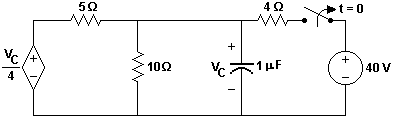
\includegraphics[width=134mm]{book_figures/p080_0.png}
\caption*{Circuit for Problem 080}
\end{figure}

Solution: Let us see:

\begin{entry}
sq\dc("e1,1,0,vc/4;r1,1,2,5;r2,2,0,10;c,2,0,10^-6;
      r3,2,3,4;e2,3,0,40"):vc
\end{entry}

We prefer to use exact values. Remember that the sign of
\code{10\^{}-6} is the negation sign, not the subtraction sign. We
press \key{ENTER}. We obtain 20 as the voltage in the capacitor.
This will be its initial condition for the simulation of the next
interval:

\begin{entry}
sq\fd("e1,1,0,vc/4,0;r1,1,2,5,0;r2,2,0,10,0;c,2,0,10^-6,20"):
sq\fd_to_tr(vc)
\end{entry}

We simulate in the frequency domain, and ask for the voltage in the
capacitor, in the time domain. We press \key{ENTER}. We obtain
\code{20*e\^{}(-250000*t)}.

This problem did not give us the initial conditions, but gave us a
way to calculate them. This problem required two simulations, one
for each interval of time.

\problem{081}

\emph{Problem: Suppose the op-amp is ideal. Find $v_o(t)$.}


% figures added 10 Sep 2026
\begin{figure}[!ht]
\centering
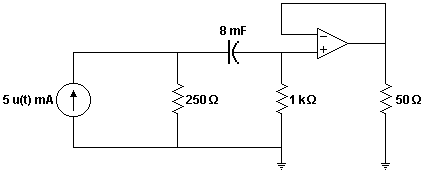
\includegraphics[width=144mm]{book_figures/p081_0.png}
\caption*{Circuit for Problem 081}
\end{figure}

Solution: The problem gives us to understand that there are no
initial conditions. Therefore, we will run only one simulation. We
simulate in the frequency domain, and ask for the output voltage, in
the time domain. We prefer to use exact values:

\begin{entry}
sq\fd("j1,0,1,5/1000,0;r1,1,0,250,0;ca,1,2,8/1000,0;
      r2,2,0,1000,0;o1,2,3,3,0;r3,3,0,50,0"):sq\fd_to_tr(v3)
\end{entry}

We press \key{ENTER}. We obtain \code{e\^{}(-t/10)}.

This problem used null initial conditions. It only required one
simulation.

\problem{082}

\emph{Problem: Suppose the op-amp is ideal. Find $v_o(t)$.}


% figures added 10 Sep 2026
\begin{figure}[!ht]
\centering
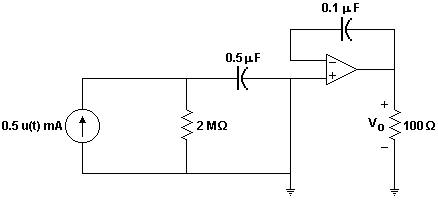
\includegraphics[width=149mm]{book_figures/p082_0.png}
\caption*{Circuit for Problem 082}
\end{figure}

Solution: This problem is like the previous one. We prefer to use
approximate values:

\begin{entry}
sq\fd("j1,0,1,.5E-6,0;r1,1,0,2E6,0;ca,1,2,.5E-6,0;o1,0,2,3,0;
      cb,2,3,.1E-6,0;r2,3,0,100,0"):sq\fd_to_tr(v3)
\end{entry}

We press \key{ENTER}. We obtain \code{5.*e\^{}(-t)-5.}

This problem used null initial conditions. It only required one
simulation.

\problem{083}

\emph{Problem: In the circuit shown, let $L = 5$~H,
$R = 8~\Omega$, $C = 12.5$~mF and $v(0^{+}) = 40$~V. Find a) $v(t)$
if $i(0^{+}) = 8$~A, b) $i(t)$ if $i_C(0^{+}) = 8$~A.}


% figures added 10 Sep 2026
\begin{figure}[!ht]
\centering
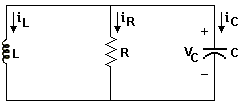
\includegraphics[width=83mm]{book_figures/p083_0.png}
\caption*{Circuit for Problem 083}
\end{figure}

Solution: The problem gives us the initial condition of the
capacitor. Then it asks us two questions. For the first question, it
also tells us the initial condition of the inductor. We simulate in
the frequency domain, and ask for the voltage in the time domain:

\begin{entry}
sq\fd("l,1,0,5,8;r,1,0,8,0;c,1,0,12.5E-3,40"):sq\fd_to_tr(v1)
\end{entry}

We press \key{ENTER}. We obtain
\code{160.*e\^{}(-8*t)-120.*e\^{}(-2*t)}. This answers question a).

For the second question, the problem does not tell us the initial
condition of the inductor, but gives us the way to find it. We
simulate in the frequency domain, using a symbolic value \code{io}
as the initial condition for the inductor, since we do not know its
numerical value. (The initial condition of the inductor that the
problem gave us earlier was valid only for question a).)

\begin{entry}
sq\fd("l,1,0,5,io;r,1,0,8,0;c,1,0,12.5E-3,40")
\end{entry}

We press \key{ENTER}. We know that the current in the capacitor is
worth 8 at $t = 0$. We ask for \code{sq\char`\\fd\_to\_tr(ic)} and
obtain a symbolic expression in terms of \code{io}. We must solve
this expression to obtain the numerical value of \code{io}. We solve
it like this: \code{solve(ans(1)=8,io)|t=0}. What we are asking is:
``Tell me how much \code{io} is worth if the current in the
capacitor, whose expression is in \code{ans(1)}, at time zero is
worth 8.'' This is a way of asking: how much must the initial
condition of the inductor be so that the current in the capacitor at
time zero is 8? We obtain: \code{io}~$= -13.$ That is the initial
condition of the inductor. Now we must find the expression for the
current in the inductor. We could simulate again, using the
numerical initial condition. But the simplest thing is to just
replace in the expression the value we found with \code{solve}. We
ask for \code{sq\char`\\fd\_to\_tr(il)|ans(1)} and obtain
\code{3.*e\^{}(-8*t)-16.*e\^{}(-2*t)}. This answers question b).

\problem{084}

\emph{Problem: Find $i_L(t)$ for $t > 0$ in the circuit shown in the
figure.}


% figures added 10 Sep 2026
\begin{figure}[!ht]
\centering
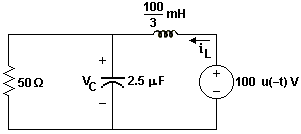
\includegraphics[width=102mm]{book_figures/p084_0.png}
\caption*{Circuit for Problem 084}
\end{figure}

Solution: We must understand the $u(-t)$ as a switch: the source is
worth 100 for $t < 0$, and worth 0 for $t > 0$. Therefore, we will
use the concept of two intervals:

\begin{entry}
sq\dc("r,1,0,50;c,1,0,2.5E-6;l,1,2,(100/3)E-3;e,2,0,100")
\end{entry}

Remember that the sign that appears in \code{E-6} is the negation
sign, not the subtraction sign. We press \key{ENTER}. Let us obtain
the initial conditions. For \code{vc} we obtain 100. For \code{il}
we obtain $-2$. We simulate in the frequency domain, and ask for the
current in the inductor, in the time domain:

\begin{entry}
sq\fd("r,1,0,50,0;c,1,0,2.5E-6,100;l,1,2,(100/3)E-3,-2;
      e,2,0,0,0"):expand(sq\fd_to_tr(il))
\end{entry}

Note that the source was given a value of 0. There were two other
alternatives: use a short circuit, or eliminate the source and
connect the inductor to the reference node. We press \key{ENTER}. We
obtain \code{.25/(e\^{}t)\^{}6000-2.25/(e\^{}t)\^{}(2000.)}. This is
the same as saying $.25e^{-6000t} - 2.25e^{-2000t}$.

\problem{085}

\emph{Problem: Find $i_s(t)$ for $t > 0$ in the circuit of the
figure if $v_s(t)$ is a) $10u(-t)$~V, b) $10u(t)$~V.}


% figures added 10 Sep 2026
\begin{figure}[!ht]
\centering
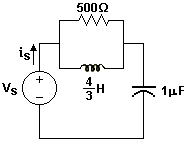
\includegraphics[width=64mm]{book_figures/p085_0.png}
\caption*{Circuit for Problem 085}
\end{figure}

Solution: Let us answer question a). We must understand the $u(-t)$
as a switch that makes the source worth 10 for $t < 0$, and 0 for
$t > 0$. Therefore, we will use the concept of two intervals:

\begin{entry}
sq\dc("e,1,0,10;r,1,2,500;l,1,2,4/3;c,2,0,1/10^6")
\end{entry}

We press \key{ENTER}. Let us obtain the initial conditions. For
\code{vc} we obtain 10. For \code{il} we obtain 0.

\begin{entry}
sq\fd("e,1,0,0,0;r,1,2,500,0;l,1,2,4/3,0;c,2,0,1/10^6,10"):
sq\fd_to_tr(-ie)
\end{entry}

We use the negative on \code{ie} because $i_s$ is defined in the
opposite sense to \code{ie}. We press \key{ENTER}. We obtain
\code{e\^{}(-500*t)/400-9*e\^{}(-1500*t)/400}. If we want to see the
answer in approximate form, instead of
\code{sq\char`\\fd\_to\_tr(-ie)}, we use
\code{expand(approx(sq\char`\\fd\_to\_tr(-ie)))}. We obtain the
expression \code{.0025/(e\^{}t)\^{}500-.0225/(e\^{}t)\^{}1500}. This
is the same as saying $.0025e^{-500t} - .0225e^{-1500t}$. This
answers question a).

Let us answer question b). We must understand the $u(t)$ as a switch
that makes the source worth 0 for $t < 0$, and 10 for $t > 0$.
Therefore, we will only need one interval, since the source is dead
before $t$. We use null initial conditions:

\begin{entry}
sq\fd("e,1,0,10,0;r,1,2,500,0;l,1,2,4/3,0;c,2,0,1/10^6,0"):
sq\fd_to_tr(-ie)
\end{entry}

We press \key{ENTER}. We obtain
\code{9*e\^{}(-1500*t)/400-e\^{}(-500*t)/400}. If we want to see the
answer in approximate form, we use the same procedure explained
above. We would obtain $.0225e^{-1500t} - .0025e^{-500t}$. This
answers question b).

\section{The (Impala) Mode}

Like the (Expert) Mode, the (Impala) Mode is a variant in the way
Symbulator solves a problem. But unlike the (Expert), which must be
activated by the user at will, the (Impala) activates itself
automatically when it is necessary.

The (Impala) Mode activates when the user enters some source whose
value is a function of time, that is, containing exponentials,
trigonometric functions, etc. Examples of these sources would be:
$100e^{-80t}$, $10e^{-t}\sin(2t + 30°)$ and others of that style.

What this mode does is write and solve the equations using the value
of the source as a simple symbolic variable, called
$\sigma$\code{name}, where \code{name} is that of the source. Once
the equations have been solved, before storing the answers, the
Impala replaces the variable $\sigma$\code{name} with the value of
the source in the frequency domain. This simple substitution saves a
considerable amount of time. In the following example, and in an
example of the next chapter, we will see the (Impala) Mode in
action. We will know this mode activates when the messages
indicating so appear on the screen.

This mode receives its name in honor of an African antelope, which
on seeing itself threatened by its predators, escapes by taking
prodigious leaps. So too Symbulator, on meeting very complex
sources, leaps, avoiding the use of their complicated value, and
solves the equations using a simple symbolic value; then it lands,
replacing the source by its complicated value in the frequency
domain.

\problem{086}

\emph{Problem: Let $v_s = 100e^{-80t}$ and $v_1(0) = 20$~V in the
circuit of the figure. a) Find $i(t)$. b) Find $v_1(t)$. c) Find
$v_2(t)$.}


% figures added 10 Sep 2026
\begin{figure}[!ht]
\centering
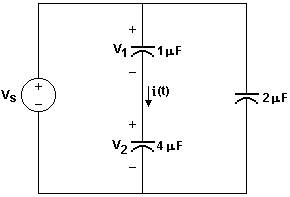
\includegraphics[width=99mm]{book_figures/p086_0.png}
\caption*{Circuit for Problem 086}
\end{figure}

Solution: The problem gives us the initial condition of the 1~µF
capacitor; however, it does not tell us those of the 4~µF and 2~µF
capacitors. Running a DC simulation of this circuit will not help us
find these initial conditions. But we can deduce them easily, using
Kirchhoff's voltage law. So, we deduce that the initial condition of
the 4~µF capacitor is 80~V, and that of the 2~µF capacitor is
100~V.

Since the problem asks us for three answers in the time domain, and
the circuit is small, we will use TR instead of FD. We will use
exact values:

\begin{entry}
sq\tr("e,1,0,100e^(-80t),0;cc1,1,2,1*10^-6,20;
      cc2,2,0,4*10^-6,80;cc3,1,0,2*10^-6,100")
\end{entry}

Note that the order in which the nodes of the capacitors have been
defined is in accordance with the polarity of the declared initial
voltage. We press \key{ENTER}. We see that the (Impala) Mode takes
part in the simulation. We ask for \code{icc1} and obtain
\code{-4*e\^{}(-80*t)/625}. We ask for \code{vcc1} and obtain
\code{80*e\^{}(-80*t)-60}. We ask for \code{vcc2} and obtain
\code{20*e\^{}(-80*t)+60}. These are the correct answers.
